\documentclass[xcolor=pdftex,x11names,table]{beamer}
\usepackage[T1]{fontenc}
\usepackage[utf8]{inputenc}
\usepackage[frenchb]{babel}
\usepackage{colortbl}

\usepackage{tikz}
\usepackage{tikz-er2}
\usepackage{pgf-umlcd}
\tikzstyle{every entity} = [top color=white, 
                            bottom color=blue!30, 
                            draw=blue!50!black!100, 
                            drop shadow]
\tikzstyle{every weak entity} = [drop shadow={shadow xshift=.7ex, shadow yshift=-.7ex}]
\tikzstyle{every attribute} = [top color=white, 
                               bottom color=yellow!20, 
                               draw=yellow, 
                               node distance=1cm, 
                               drop shadow]
\tikzstyle{every relationship} = [top color=white, 
                                  bottom color=yellow!20,  
                                  draw=yellow, 
                                  drop shadow]
\tikzstyle{every isa} = [draw=blue!50!black!100]
\usetikzlibrary{decorations,arrows,shapes,backgrounds,shadows,calc}
\usetikzlibrary{positioning}
\usetikzlibrary{automata}

\usepackage{ifthen}
\usepackage{changepage}

\usepackage{listings}

\usepackage{textcomp}
 
\definecolor{gray}{gray}{0.5} 
\lstnewenvironment{code_xml}[1][]{ 
    \lstset
      { 
        language=XML,
        inputencoding=utf8,
        basicstyle=\ttfamily, 
        showspaces=false,
        showstringspaces=false,
        showtabs=false,
        frame=single,
        morecomment=[s]{<!--}{-->},
        commentstyle=\itshape\color{gray},
        stringstyle=\color{blue},
        keywordstyle=\color{red},
        markfirstintag=true,
        upquote=true
      } 
}{}

\setbeamertemplate{blocks}[rounded][shadow=true]

\title[Persistance des données]{Persistance des données en Java}
%\author{Sébastien NEDJAR}
%\institute{IUT d'Aix-en-Provence}
\date{}

\usecolortheme{crane}
\definecolor{couleurprincipale}{HTML}{FFCC00}

\AtBeginSection[]
{
  \begin{frame}<beamer>
    \frametitle{Plan}
    \tableofcontents[currentsection,hideothersubsections]
  \end{frame}
}

\begin{document}
  \lstset{             
    %breaklines=true,                                     % line wrapping on
    %frame=ltrb,
    %samepage=true,
    language=Java,
    basicstyle=\normalsize,
    frameround=ftft,
    keywordstyle=\ttfamily\color{SeaGreen4},
    identifierstyle=\ttfamily\bfseries\color{RoyalBlue4},
    commentstyle=\color{RoyalBlue3},
    stringstyle=\ttfamily,
    showstringspaces=false,
    tabsize=2,  
  }

  % For every picture that defines or uses external nodes, you'll have to
  % apply the 'remember picture' style. To avoid some typing, we'll apply
  % the style to all pictures.
  \tikzstyle{every picture}+=[remember picture]
  \tikzstyle{na} = [baseline=-.5ex]

  % ---------- Titre -----------
  \begin{frame}
  \titlepage
  \end{frame}
  % ----------------------------
  \section{Présentation du cours}

  \section{Persistance fondée sur les concepts relationnels : JDBC}
  	\subsection{Introduction}
    \subsection{Traitement d’une requête SQL}
		\subsection{Traitement d’un ordre de modification des données}
		\subsection{Traitement d’un appel de procédure stockée}
		\subsection{Les Meta Informations}
		\subsection{Conclusion Temporaire}
    
        
  \section{Persistance fondée sur les concepts objets}
  	\subsection{Introduction}
  	\begin{frame}
    \frametitle{Correspondance Objet/Relationnel}
		  \begin{itemize}
		  	\item Ce cours explique les problèmes de base qui se posent quand on veut faire correspondre :\\
				les données contenues dans un modèle objet avec les données contenues dans une base de données relationnelle
		  	\item Dans le TP1 vous avez vu en partie comment faire correspondre manuellement un modèle relationnel 
		  	avec un modèle objet.
		  	\item Dès qu’un modèle objet est complexe (de l’héritage et beaucoup d’associations), il n’est pas simple de lui 
		  	faire correspondre un modèle relationnel.
		  	\item Nécessité d'un outil pour définir le plus simplement possible cette correspondance : JPA.
		  \end{itemize}	
   	\end{frame}
   	
   	\subsection{Comparaison modèle objet / modèle relationnel}
   	\begin{frame}
    \frametitle{Quelques problèmes du passage Relationnel $\leftrightarrow$ Objet}
		  \begin{itemize}
		  	\item Identité des objets (pas de notion de clef)
		  	\item Traduction des différents types d'associations (hiérarchiques, non hiérarchiques, ...)
		  	\item Navigation entre les objets (restriction de la navigabilité)
		  	\item Traduction de l’héritage
		  \end{itemize}	
   	\end{frame}

   	\begin{frame}
    \frametitle{Problème de base}
		  \begin{itemize}
		  	\item Un objet a une structure complexe qui peut être représentée par un graphe.
		  	\item Le plus souvent ce graphe est un arbre dont la racine correspond à l’objet et les fils correspondent aux 
		  	valeurs de ses variables d’instance.
		  	\item Il faut « aplatir » ce graphe pour le ranger dans la base de données relationnelle sous une forme tabulaire.
		  	\item Le chargement d'un seul objet peut demander de récupérer un grand nombre de tuples situés dans des 
		  	relations différentes.
		  \end{itemize}	
   	\end{frame}

   	\begin{frame}
    \frametitle{Traduction d’une classe en une relation}
		  \begin{itemize}
		  	\item Dans les cas les plus simples (lorsque toutes les données membres ont un type simple) une classe est 
		  	traduite en une relation.
		  	\item Chaque objet est conservé dans un tuple de la relation et les données membres sont traduites en attributs.
		  	\item Exemple : la classe Personne est traduite par la relation : \\ \texttt{Personne(\underline{IdPer}, Nom, Prénom, Age, Sexe)} 
		  \end{itemize}	
		  
		  \begin{center}
		  \begin{tikzpicture}[]
				\begin{class}[text width=3.5cm]{Personne}{0,0}
				\attribute{-idPer : int }
				\attribute{-nom : String}
				\attribute{-prénom : String}
				\attribute{-age : int}
				\attribute{-sexe : String}
				\end{class}
			\end{tikzpicture}
			\end{center}
   	\end{frame}


   	\begin{frame}
    \frametitle{Identification dans le monde Objet}
		  \begin{itemize}
		  	\item Tout objet est identifiable simplement dans les langages objets par l'adresse de son emplacement mémoire, 
		  	indépendamment des données qu’il contient. 
		  	\item Deux objets distincts peuvent avoir exactement les mêmes valeurs pour leurs propriétés.
		  	\item Il y a donc une différence conceptuelle entre deux objets qui sont égaux (\lstinline$o1.equals(o2)$) et deux objets 
		  	qui sont identiques (\lstinline$o1==o2$)
		  \end{itemize}	
   	\end{frame}

   	\begin{frame}
    \frametitle{Identification dans le monde relationnel}
		  \begin{itemize}
		  	\item Seules les valeurs des attributs peuvent servir à identifier un tuple.
		  	\item Si deux tuples ont les mêmes valeurs, il est impossible de les différencier. 
		  	Ils sont donc considérés identiques.
		  	\item Une clef primaire est le plus petit ensemble d'attributs permettant d'identifier de manière non équivoque 
		  	tous les tuples d'une relation.
				\item Toute relation doit donc comporter une clé primaire pour identifier facilement un tuple parmi tous les 
				autres tuples de la même relation.
				\item Deux tuples égaux étant considéré identique, une relation ne contiendra pas de doublon.
		  \end{itemize}	
   	\end{frame}

   	\begin{frame}
    \frametitle{Clef primaire pour les objets}
		  \begin{itemize}
		  	\item Pour des raisons d'efficacité, on fait en sorte que les relations aient une clef simple(un Id numérique).
		  	\item Cet attribut devra être représenté dans une donnée membre de chaque classe.
		  	\item En effet, il pourra être utilisé par le code pour un accès rapide aux données ou pour aider à gérer 
		  	le mapping objet-relationnel.
				\item Cette propriété servant à l'identification d'un objet, on ne doit pas pouvoir la modifier après la création de 
				l'objet (pas de méthode \lstinline$setId()$ publique).
		  \end{itemize}	
   	\end{frame}
   	
   	\begin{frame}
    \frametitle{Problème des duplications}
		  \begin{itemize}
		  	\item Une même ligne de la base de données ne doit pas être représentée par plusieurs objets en 
		  	mémoire (ou alors le code doit le savoir et en tenir compte).
		  	\item Si elle n’est pas gérée, cette situation peut conduire à des pertes ou des incohérences de données.
				\item Par exemple, Un objet $p_1$ de la classe \texttt{Produit} de code 1003 est chargé en mémoire à l’occasion
							d’une navigation à partir d’une ligne de \texttt{Facture}.
				\item On peut retrouver le même produit en navigant depuis une autre facture, ou en cherchant tous les produits 
				qui vérifient un certain critère.
			\end{itemize}	
   	\end{frame}
   	\begin{frame}
    \frametitle{Problème des duplications (suite)}
		  \begin{itemize}				
				\item Si l'on crée en mémoire centrale un autre objet $p_2$ indépendant du premier objet $p_1$ déjà créé, 
				il peut arriver que les deux objets soient modifiés en même temps par deux parties du code. Dans ce cas on ne 
				peut plus savoir lequel des objets est dans l'état correct.
				\item Pour éviter ce problème, on doit généralement conserver en mémoire un "cache" des objets déjà chargés.
				\item Ainsi si l'on à besoin d'un objet, on vérifie toujours s'il en existe pas déjà un qui possède la même 
				identité dans le cache.
				\item C'est le pattern "Unit of Work" de Martin Fowler (Oncle Bob).
		  \end{itemize}	
   	\end{frame}

		\begin{frame}
    \frametitle{Objets « intégrés »}
		  \begin{itemize}
				\item Les instances de certaines classes peuvent être sauvegardées dans la même relation qu’une autre classe.
				\item Ces instances sont appelées des objets intégrés (embedded en anglais, qui signifie intégré, imbriqué) 
				et ne nécessitent pas d’identificateur « clé primaire ».
				\item Par exemple, une classe \texttt{Adresse} peut ne pas avoir de correspondance sous la forme d’une relation
							séparée dans le modèle relationnel.
				\item Les attributs de la classe \texttt{Adresse} sont intégrés dans la relation qui représente la classe \texttt{Client}
				\item Les objets de la classe \texttt{Adresse} n’ont pas d’identification liée à la base de données.
		  \end{itemize}	
   	\end{frame}

		\begin{frame}
    \frametitle{Les associations en objet}
    	Dans le code objet une association peut être représentée par :
		  \begin{itemize}
		  	\item Une variable d’instance référençant l’objet associé (association 1:1 ou N:1)
		  	\item Une variable d’instance de type collection ou map contenant les objets associés (association 1:N ou M:N)
		  	\item Une classe « association » (M:N)
		  \end{itemize}
		  Par exemple pour une association 1:N :
		  \begin{block}{}
    		\lstinline$class Departement \{$\\
    		\lstinline$\ \ private Collection<Employe> employes;$\\
    		\lstinline$\ \ ...$\\
    		\lstinline$\}$
    	\end{block}
    	\begin{block}{}
    		\lstinline$class Employe \{$\\
    		\lstinline$\ \ private Departement departement;$\\
    		\lstinline$\ \ ...$\\
    		\lstinline$\}$
    	\end{block}
   	\end{frame}
 
		\begin{frame}
    \frametitle{Association en relationnel}
    Dans le monde relationnel, une association peut être représentée par :
		  \begin{itemize}
		  	\item une ou plusieurs clés étrangères (associations hiérarchique 1:1, N:1 ou 1:N).
				\item une table association (associations non hiérarchique M:N le plus souvent)
		  \end{itemize}	
   	\end{frame}

		\begin{frame}
    \frametitle{Navigabilité des associations}
		  \begin{itemize}
		  	\item Dans un modèle objet, une association peut être bi ou unidirectionnelle.
		  	\item Exemple d’association unidirectionnelle : la classe \texttt{Employé} a une variable d’instance
							donnant son département mais la classe \texttt{Département} n’a pas de collection d’employés.
				\item En partant d’un département, on n’a alors pas de moyen simple de retrouver ses employés.
				\item Dans le modèle relationnel, toutes les associations sont bidirectionnelles.
				\item La navigation se fait grâce à des jointures. 
		  \end{itemize}	
   	\end{frame}

		\begin{frame}
    \frametitle{Objet dépendant}
		  \begin{itemize}
		  	\item Un objet dont le cycle de vie dépend du cycle de vie d’un autre objet auquel il est associé, appelé objet propriétaire.
				\item Aucun autre objet que le propriétaire ne doit avoir de référence directe vers un objet dépendant.
				\item En ce cas, la suppression de l’objet propriétaire doit déclencher la suppression des objets qui en dépendent (déclenchement « en cascade »).
				\item Par exemple, une ligne de facture ne peut exister qu’associée à une (en-tête de) facture.
				\item Si on supprime une facture, toutes les lignes de la facture doivent être supprimées.
		  \end{itemize}	
   	\end{frame}

		\subsection{Framework de mapping objet/relationnel: JPA2}
		\begin{frame}[allowframebreaks]
    \frametitle{Framework de mapping objet/relationnel}
    La correspondance entre le modèle objet et le modèle relationnel n’est pas une tâche facile. Il est nécessaire de 
    posséder des outils pour maîtriser cette tâche. L'outil aura les qualités suivantes :
		  \begin{itemize}
		  	\item \textbf{Objet et pas relationnel} : L'application doit être écrite en terme de domaine métier en ne pas 
		  	se borner à une modélisation relationnelle. Donc on doit pouvoir développer en faisant abstraction des concepts 
		  	relationnels comme les clefs, les relations ou les tuples.
		  	\item \textbf{Facile mais pas inculte} : L'outil de mapping doit aider le développeur à interagir avec un SGBD-R 
		  	pas le rendre ignorant des mécanismes sous-jacents. Pour bien utiliser la persistance, il faut comprendre le 
		  	fonctionnement des BD.   
		  	\item \textbf{Non intrusif mais pas transparent} : Il n'est pas raisonnable de demander à la persistance d'être 
		  	totalement transparente (automatique) car l'application doit toujours garder le contrôle du cycle de vie de ses objets. 
		  	Néanmoins, il ne faut pas non plus que le code soit trop profondément dépendant de l'outil de persistance car le 
		  	code métier (principal) serait noyé au milieu du code de persistance (juste utilitaire).
		  	\item \textbf{Suffisant mais pas excessif} : Le développeur d'une application à des problèmes à résoudre et il 
		  	souhaite un outil assez complet pour remplir tous ses besoins même les plus complexes. Mais il ne souhaite pas 
		  	devoir configurer lourdement un outil pour ses besoins les plus simples.
		  	\item \textbf{Local mais mobile} : Les objets persistants ne doivent pas être des vrais objets distribués mais il 
		  	faut pouvoir en récupérer une copie peu importe l'endroit ou l'on se trouve.  
		  \end{itemize}	
   	\end{frame}

		\begin{frame}
    \frametitle{JPA2}
		  \begin{itemize}
		  	\item JPA2 (Java Persistence API version 2.0) est un standard pour la persistance des objets en Java.
		  	\item JPA2 est le plus souvent utilisé dans le contexte d’un serveur d’applications (Java EE).
				\item Ce cours étudie l’utilisation de JPA2 par une application classique (Java SE).
				\item Comme pour JDBC, l’utilisation de JPA2 nécessite un fournisseur de persistance qui 
				implémente les classes et méthodes de l’API.
				\item Nombreuses implémentations commerciale et libre de cette spécification : Hibernate, TopLink, OpenJPA, EclipseLink, ...
		  \end{itemize}	
   	\end{frame}

  \begin{frame}[allowframebreaks]
    \frametitle{Qualités de JPA}
    Le modèle de JPA est simple et élégant, puissant et flexible. Les points forts de cette API sont les suivants : 
    \begin{itemize}
		  \item Les opérations principales de l'API sont contenues dans un petit nombre de classes faciles à apprendre et à comprendre.
		  \item La persistance est basée uniquement sur des POJO (bons vieux objets java) donc il n'est pas nécessaire d'étendre ou implémenter 
		  quoi que ce soit pour gérer la persistance. Globalement tout objet java avec un constructeur par défaut peut devenir persistant.
		  \item JPA est non intrusive, les objets métier n'ont pas besoin d'être modifié pour devenir persistant.
		  \item Un langage de requête Objet proche du SQL permet de facilement récupérer les objets correspondant à des critères donnés.
		  \item La configuration est relativement simple, par défaut JPA propose une convention pouvant convenir à la majorité des projets. 
		  On ne doit configurer l'outil que si la convention ne s'adapte pas à notre cas.
		  \item JPA n'utilisant que des spécifications disponibles dans Java SE, il est relativement simple à tester.
		\end{itemize}
   \end{frame}

	 \lstset{basicstyle=\scriptsize,language=Java}
   \begin{frame}
     \frametitle{Entités}
     Pour JPA, une entité est une classe dont les instances peuvent être rendues persistantes. \pause
     \begin{block}{}\footnotesize
    	\lstinline$public class Employe \{$\\
    	\lstinline$\ \ \ \ private int id;$\\
    	\lstinline$\ \ \ \ private String nom;$\\
    	\lstinline$\ \ \ \ private long salaire;$\\
    	\lstinline$\ \ \ \ private Departement departement;$\\
    	\lstinline$\ \ \ \ public Employe() \{\}$\\
    	\lstinline$\ \ \ \ public Employe(int id) \{ this.id = id; \}$\\
    	\lstinline$\ \ \ \ public int getId() \{ return this.id; \}$\\
    	\lstinline$\ \ \ \ private void setId(int id) \{ this.id = id; \}$\\
    	\lstinline$\ \ \ \ public String getNom() \{ return this.nom; \}$\\
    	\lstinline$\ \ \ \ public void setNom(String nom) \{ this.nom = nom; \}$\\
    	\lstinline$\ \ \ \ public int getSalaire() \{ return this.salaire; \}$\\
    	\lstinline$\ \ \ \ public void setSalaire(long salaire) \{ this.salaire =salaire; \}$\\
    	\lstinline$\ \ \ \ public Departement getDepartement() \{ return this.departement; \}$\\
    	\lstinline$\ \ \ \ public void setDepartement(Departement dept) \{ this.departement = dept; \}$\\
    	\lstinline$\}$
		 \end{block}
  \end{frame}
  
  \begin{frame}
     \frametitle{Entités}
     Pour transformer \texttt{Employe} en entité il suffit de lui rajouter les annotations suivantes :  \pause
     \begin{block}{}\footnotesize
      \lstinline$@Entity$\\
    	\lstinline$public class Employe \{$\\
    	\lstinline$\ \ \ \ @Id private int id;$\\
    	\lstinline$\ \ \ \ private String nom;$\\
    	\lstinline$\ \ \ \ private long salaire;$\\
    	\lstinline$\ \ \ \ @ManyToOne private Departement departement;$\\
    	\lstinline$\ \ \ \ public Employe() \{\}$\\
    	\lstinline$\ \ \ \ public Employe(int id) \{ this.id = id; \}$\\
    	\lstinline$\ \ \ \ public int getId() \{ return this.id; \}$\\
    	\lstinline$\ \ \ \ private void setId(int id) \{ this.id = id; \}$\\
    	\lstinline$\ \ \ \ public String getNom() \{ return this.nom; \}$\\
    	\lstinline$\ \ \ \ public void setNom(String nom) \{ this.nom = nom; \}$\\
    	\lstinline$\ \ \ \ public int getSalaire() \{ return this.salaire; \}$\\
    	\lstinline$\ \ \ \ public void setSalaire(long salaire) \{ this.salaire =salaire; \}$\\
    	\lstinline$\ \ \ \ public Departement getDepartement() \{ return this.departement; \}$\\
    	\lstinline$\ \ \ \ public void setDepartement(Departement dept) \{ this.departement = dept; \}$\\
    	\lstinline$\}$
		 \end{block}
  \end{frame}
  \lstset{basicstyle=\normalsize}
  \begin{frame}
    \frametitle{Entité}
    \begin{itemize}
		  \item Par convention cette entité sera associée à la relation \texttt{EMPLOYE}.
		  \item les propriétés seront stockés dans des attributs de même nom avec le type SQL adapté.
		  \item L'annotation \lstinline$@Entity$ permet d'indiquer à JPA que la classe pourra être rendue persistante.
		  \item L'annotation \lstinline$@Id$ précise la donnée membre qui sera utilisée comme identifiant (clef primaire).
		  \item L'annotation \lstinline$@ManyToOne$ précise que la donnée membre \texttt{departement} est une association hiérarchique de type N:1.
		  \item Pour sauvegarder l'état d'une instance de \texttt{Employe}, il faudra faire un appel à l'API JPA. 
		\end{itemize}
  \end{frame}
  \begin{frame}
    \frametitle{\texttt{EntityManager}}
    Pour rendre persistant des objets, il faut utiliser les classes fournies par JPA. Parmi toutes ces classes la plus 
    importante est le Gestionnaire d'entité \texttt{EntityManager}.
    \begin{itemize}
		  \item Le gestionnaire d’entités (GE) est l’interlocuteur principal pour le développeur.
		  \item Il fournit les méthodes pour gérer les entités : les rendre persistantes, les supprimer de la
			base de données, retrouver leurs valeurs dans la base, etc.
			\item Le GE est créé par la classe \texttt{EntityManagerFactory} en utilisant l'unité de persistance définie dans 
			le fichier \texttt{persistence.xml}
			\item On peut configurer l'unité de persistance pour que les relations soient automatiquement générées 
			au premier lancement de l'application.
		\end{itemize}
  \end{frame}

  \begin{frame}
    \frametitle{Récupération d'un gestionnaire d’entités}
    Avant de récupérer le gestionnaire d'entité, il faut construire la fabrique de gestionnaire d'entité associée à notre unité de persistance (équivalent d'une 
    connexion en JDBC).
    \begin{block}{}
    	\lstinline$EntityManagerFactory emf = $\\
    	\lstinline$\ \ \ \ Persistence.createEntityManagerFactory("persUnit");$\\
		\end{block}
		Le nom passé en paramètre est celui de l'unité de persistance définie dans le fichier \texttt{persistence.xml}.
		À partir de cette fabrique on peut donc construire notre GE :
		\begin{block}{}
    	\lstinline$EntityManager em = emf.createEntityManager();$\\
		\end{block}
		Grâce à cet objet nous allons pouvoir commencer à travailler avec les entités persistantes.
  \end{frame}

  \begin{frame}
    \frametitle{Persistance d'une entité}
    \begin{itemize}
		  \item Par défaut un objet de la classe \texttt{Employe} n'est pas persistant. C'est une entité dite \texttt{transient}.
		  \item Pour rendre une entité \texttt{transient} persistante, il faut l'enregistrer au près du GE avec la méthode \lstinline$persist()$.
		  \item Une fois persistant, l'objet est transformé en un tuple de la relation \texttt{EMPLOYE}.
				\begin{block}{}
					\lstinline$Employe emp = new Employe(123);$\\
					\lstinline$em.persist(emp);$\\
				\end{block}
			\item Cette méthode peut lever une exception non contrôlée du type \texttt{PersistenceException}.
		\end{itemize}
  \end{frame}
  \begin{frame}
    \frametitle{Persistance d'une entité}
    \begin{itemize}
		  \item L'exemple ci-dessous incorpore ces éléments dans une méthode permettant de créer directement des entités 
		  persistantes. On supposera que cette méthode appartient à une classe ayant le GE en donnée membre.
				\begin{block}{}
					\lstinline$public Employe createEmploye(int id,$\\
					\lstinline$\ \ \ \ \ \ \ \ \ \ \ \ \ \ \ \ \ \ \ \ String nom, long salaire) \{$\\
					\lstinline$\ \ \ \ Employe emp = new Employe(id);$\\
					\lstinline$\ \ \ \ emp.setNom(nom);$\\
					\lstinline$\ \ \ \ emp.setSalaire(salaire);$\\
					\lstinline$\ \ \ \ em.persist(emp);$\\
					\lstinline$\ \ \ \ return emp;$\\
					\lstinline$\}$\\
				\end{block}
		\end{itemize}
  \end{frame}
  
  \begin{frame}
    \frametitle{Rechercher des entités}
    \begin{itemize}
		  \item Une fois les entités dans la base de données, l'étape suivante est de pouvoir la retrouver ultérieurement.
		  \item Pour retrouver une entité à partir de son identifiant, il suffit d'appeler la méthode \texttt{find()} du GE. 
				\begin{block}{}
						\lstinline$Employe emp = em.find(Employe.class, 123);$\\
				\end{block}
			\item L'entité retourné par le GE est une entité gérée (managed).
			\item Si le GE ne trouve aucune entité correspondant au paramètre passé à la méthode \texttt{find()}, il retourne 
			simplement la valeur \texttt{null}.
			\item La méthode de recherche d'un employé :
				\begin{block}{}
					\lstinline$public Employe findEmploye(int id) \{$\\
					\lstinline$\ \ \ \ return em.find(Employe.class, id);$\\
					\lstinline$\}$\\
				\end{block}
		\end{itemize}
  \end{frame}
  \begin{frame}
    \frametitle{Supression d'une entité}
    \begin{itemize}
		  \item Généralement les données ne sont que rarement totalement effacées de la BD. Le stockage coûtant peu, 
		  les entités seront archivé au lieu d'être supprimées.
		  \item Pour qu'un objet puisse être supprimé, il faut que ce soit une entité gerée (managed).
		  	\begin{block}{}
						\lstinline$Employe emp = em.find(Employe.class, 123);$\\
						\lstinline$em.remove(emp);$\\
				\end{block}
		  \item La methode suivante supprime un employé à partir de son Id:
		  	\begin{block}{}
					\lstinline$public void removeEmploye(int id) \{$\\
					\lstinline$\ \ \ \ Employe emp = em.find(Employe.class, id);$\\
					\lstinline$\ \ \ \ if (emp != null)$\\
					\lstinline$\ \ \ \ \ \ \ \ em.remove(emp);$\\
					\lstinline$\}$\\
				\end{block}
		\end{itemize}
  \end{frame}
  
  \begin{frame}[allowframebreaks]
    \frametitle{Mise à jour d'une entité}
    \begin{itemize}
		  \item Il existe plusieurs manière de mettre à jour une entité avec JPA, nous allons voir la plus commune : 
		  nous avons une entité gerée (managed) et nous voulons la modifier.
		  	\begin{block}{}
						\lstinline$Employe emp = em.find(Employe.class, 123);$\\
						\lstinline$emp.setSalaire(emp.getSalaire()+1000);$\\
				\end{block}
			\item Contrairement aux autres modifications, la mise à jour ne passe pas par le GE. L'objet est modifié et ses 
			changements sont directement répercutés dans la BD.
			\item Ceci est possible car \texttt{emp} n'est pas une simple instance de \texttt{Employe} mais une entité gérée.
			Le GE est donc informé dès qu'une modification est faire à l'entité et il exécute directement l'ordre SQL \texttt{Update}. 
		  \item La methode suivante augmente le salaire de l'employé d'identifiant \texttt{id} d'un montant \texttt{raise} :
		  	\begin{block}{}
					\lstinline$public void raiseEmployeSalaire(int id, long raise) \{$\\
					\lstinline$\ \ \ \ Employe emp = em.find(Employe.class, id);$\\
					\lstinline$\ \ \ \ if (emp != null) \{$\\
					\lstinline$\ \ \ \ \ \ \ \ emp.setSalaire(emp.getSalaire() + raise);$\\
					\lstinline$\ \ \ \ \}$\\
					\lstinline$\ \ \ \ return emp;$\\
					\lstinline$\}$\\
				\end{block}
		\end{itemize}
  \end{frame}

	\begin{frame}
    \frametitle{Transaction}
    \begin{itemize}
      \item Pour le moment tous nos exemples, ne se sont pas préoccupés des transactions.
      \item Par hypothèse pourtant toutes nos méthodes d'exemple mis à part \texttt{findEmploye()} 
      devraient se trouver dans une transaction pour garantir l'intégrité des données modifiées.
      \item Le GE nous permet grâce à la méthode \texttt{getTransaction()} de récupérer une  transaction.
      \item La méthode \texttt{begin()} permet de démarrer la transaction, et la méthode \texttt{commit()} permet 
      de la valider.
      	\begin{block}{}
      		\lstinline$em.getTransaction().begin();$\\
					\lstinline$Employe emp = CreateEmploye(123,"Anne Onyme", 45000);$\\
      		\lstinline$em.getTransaction().commit();$\\
				\end{block}
    \end{itemize}
  \end{frame}
  
  \begin{frame}[allowframebreaks]
    \frametitle{Requête JPQL}
    \begin{itemize}
      \item Généralement les développeurs connaissent bien le SQL. Pour interroger la BD d'une manière plus "objet", JPA 
      met à disposition un langage de requête proche de SQL, le JPQL (Java Persistence Query Language).
      \item Une requête sera matérialisée par un objet du type \texttt{Query} ou \texttt{TypedQuery}. Elle sera 
      construit à partir du GE.
      \item Une requête  statique est définie par des annotations directement dans la classe. Elles sont vérifiées à la 
      compilation.
      \item Une requête dynamique est construite à l'exécution dans une chaîne de caractère. Elles ne sont vérifiées 
      qu'à l'exécution, donc elles peuvent échouer si elle sont incorrectes.
        \begin{block}{}
      		\lstinline$TypedQuery<Employe> q = em.createQuery($\\
      		\lstinline$\ \ \ \ \ \ \ \ \ \ \ \ \ "SELECT e FROM Employe e", Employe.class);$\\
					\lstinline$List<Employe> listEmp = q.getResultList();$\\
				\end{block}
			\item La methode suivante revoie la liste de tous les employés :
		  	\begin{block}{}
					\lstinline$public List<Employe> findAllEmploye() \{$\\
      		\lstinline$\ \ \ \ TypedQuery<Employe> q = em.createQuery($\\
      		\lstinline$\ \ \ \ \ \ \ \ \ \ \ \ \ "SELECT e FROM Employe e", Employe.class);$\\
					\lstinline$\ \ \ \ return q.getResultList();$\\
					\lstinline$\}$\\
				\end{block}
    \end{itemize}
  \end{frame}
  
  \begin{frame}
  \frametitle{Unité de persistance : persistence.xml}
		\begin{itemize}
      \item Les paramètres de la connexion à la base de données sont définies dans le fichier \texttt{persistence.xml}.
      Ce fichier doit être situé dans le dossier \texttt{META-INF} du jar de l'application.
      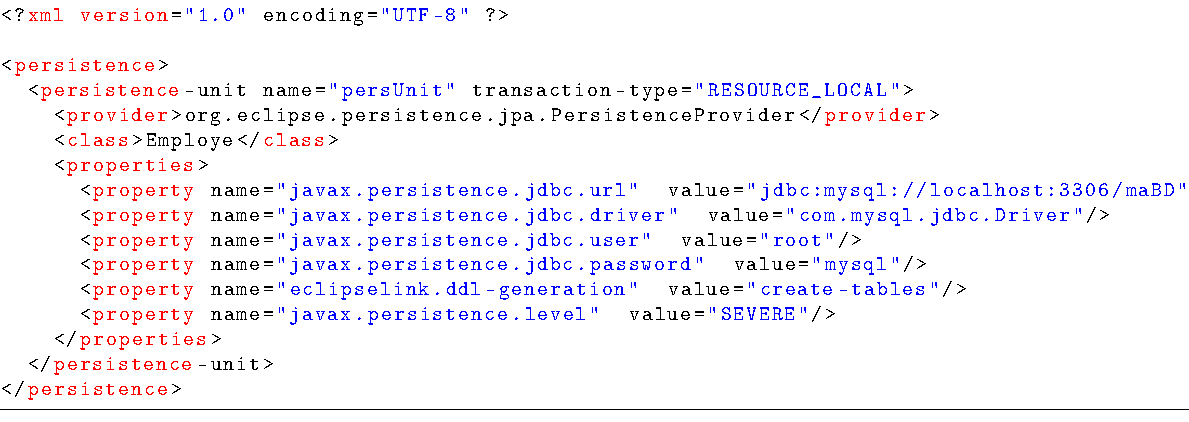
\includegraphics[width=\linewidth]{persistence.pdf}
      \item Le paramètre \texttt{" eclipselink.ddl-generation"} demande à notre implémentation de JPA de générer à notre 
      place le code sql.
    \end{itemize}
  \end{frame}

  \begin{frame}
    \frametitle{Construction d'un DAO avec JPA}
    En réunissant toute les méthodes écrite précédemment, on constate la facilité d'écriture d'un DAO à partir de JPA.
    \begin{block}{}
      \lstinline$public class DAOEmploye \{$\\
      \lstinline$private EntityManager em;$\\
      \lstinline$private DAOEmploye(String persistUnit);$\\
      \lstinline$public Employe createEmploye(int id,$\\
			\lstinline$\ \ \ \ \ \ \ \ \ \ \ \ \ \ \ \ \ \ \ \ String nom, long salaire);$\\
			\lstinline$public Employe findEmploye(int id);$\\
			\lstinline$public List<Employe> findAllEmploye();$\\
			\lstinline$public void removeEmploye(int id);$\\
			\lstinline$public void raiseEmployeSalaire(int id, long raise);$\\
			
			\lstinline$public static DAOEmploye createDAOEmploye();$\\
			\lstinline$\}$\\
    \end{block}
  \end{frame}  
  
  \begin{frame}
    \frametitle{Conclusion}
    \begin{itemize}
      \item Ce cours est une introduction rapide au monde des ORM. Cette problématique est complexe et elle mériterait 
      beaucoup plus de temps pour être abordée complètement.
      \item En TP nous allons, si le temps nous le permet, découvrir plusieurs outils Java supplémentaires pour mieux gérer nos projets :
          \begin{itemize}
      			\item Maven pour gérer le cycle de construction d'un projet (compilation, gestion des dépendance, packaging automatique,...)
      			\item JUnit pour écrire le code testant tous les modules que l'on développe pour éviter d'introduire de nouveaux bug lors de 
      			la modification du code.
      			\item DBUnit qui est un framework de test unitaire pour tester le code de la couche de persistance.
      			\item Git pour gérer facilement les évolutions de notre base de code lorsque l'on travaille à plusieurs. 
    			\end{itemize}
    \end{itemize}
  \end{frame}
  
\end{document}

